\documentclass[handout]{beamer}
%\documentclass[compress]{beamer}

%\documentclass{beamer}
\usepackage[T1]{fontenc}
\usepackage{pifont}
\usepackage{threeparttable}
\usepackage{subcaption}
\usepackage{tikz-qtree}
\usepackage{listings}
\usepackage[american]{babel}
\usepackage{csquotes}
\usepackage[style=apa, backend=biber]{biblatex}
\usepackage{tikz}
\usepackage{multicol}
\usepackage{booktabs}
\usepackage{graphicx}
\usepackage{neuralnetwork}
\usepackage{hyperref}

\usepackage{minted}
\definecolor{listingbg}{rgb}{0.87,0.93,1}
\setminted[python]{
breaklines,
linenos,
fontsize=\scriptsize,
frame=single,
xleftmargin=0pt}

\hypersetup{
    pdfborder={0 0 0},
    colorlinks=true,
}
\usetheme[block=fill,subsectionpage=progressbar,sectionpage=progressbar]{metropolis} 

\definecolor{Purple}{HTML}{911146}
\definecolor{Orange}{HTML}{CF4A30}

\setbeamercolor{alerted text}{fg=Orange}
\setbeamercolor{frametitle}{bg=Purple}

\setbeamercovered{still covered={\opaqueness<1->{5}},again covered={\opaqueness<1->{100}}}

\lstset{
    basicstyle=\scriptsize\ttfamily,
    columns=flexible,
    breaklines=true,
    numbers=left,
    %stepsize=1,
    numberstyle=\tiny,
    backgroundcolor=\color[rgb]{0.85,0.90,1}
}

\lstnewenvironment{lstlistingoutput}{\lstset{
        basicstyle=\footnotesize\ttfamily,
        columns=flexible,
        breaklines=true,
        numbers=left,
        %stepsize=1,
        numberstyle=\tiny,
        backgroundcolor=\color[rgb]{.7,.7,.7}}}{}


\lstnewenvironment{lstlistingoutputtiny}{\lstset{
        basicstyle=\tiny\ttfamily,
        columns=flexible,
        breaklines=true,
        numbers=left,
        %stepsize=1,
        numberstyle=\tiny,
        backgroundcolor=\color[rgb]{.7,.7,.7}}}{}

\renewcommand*{\bibfont}{\tiny}

\makeatletter
\setbeamertemplate{headline}{%
    \begin{beamercolorbox}[colsep=1.5pt]{upper separation line head}
    \end{beamercolorbox}
    \begin{beamercolorbox}{section in head/foot}
        \vskip2pt\insertnavigation{\paperwidth}\vskip2pt
    \end{beamercolorbox}%
    \begin{beamercolorbox}[colsep=1.5pt]{lower separation line head}
    \end{beamercolorbox}
}
\makeatother

\newcommand{\question}[1]{
    \begin{frame}[plain]
        \begin{columns}
            \column{.4\textwidth}
            \makebox[\columnwidth]{
                
\includegraphics[width=\columnwidth,height=\paperheight,keepaspectratio]{mannetje.png}}
            \column{.6\textwidth}
            \large
            \textcolor{orange}{\textbf{\emph{#1}}}
        \end{columns}
    \end{frame}}

\newcommand{\instruction}[1]{\emph{\textcolor{gray}{[#1]}}}

\addbibresource{../resources/literature.bib}
\graphicspath{{../resources/pictures/}}

\title[Computational Communication Science 2]{\textbf{Computational Communication Science 2} \\Week 1 - Online Lecture\\ »Introduction \& Lift Off«}
\author[Anne Kroon, Marthe Möller]{Anne Kroon \\ Marthe Möller ~ \\ \footnotesize{a.c.kroon@uva.nl, @annekroon} \\a.m.moller@uva.nl, @marthemoller }
\date{April 1, 2024}
\institute[Digital Society Minor, University of Amsterdam]{Digital Society Minor, University of Amsterdam}

\begin{document}
	\begin{frame}{}
		\titlepage
	\end{frame}
	
\begin{frame}{Today}
	\tableofcontents
\end{frame}

\section[The people]{Introducing\ldots the people}

\begin{frame}{Introducing\ldots \huge{Marthe}} 
	\begin{columns}
		\column{.3\textwidth}
		\makebox[\columnwidth]{
			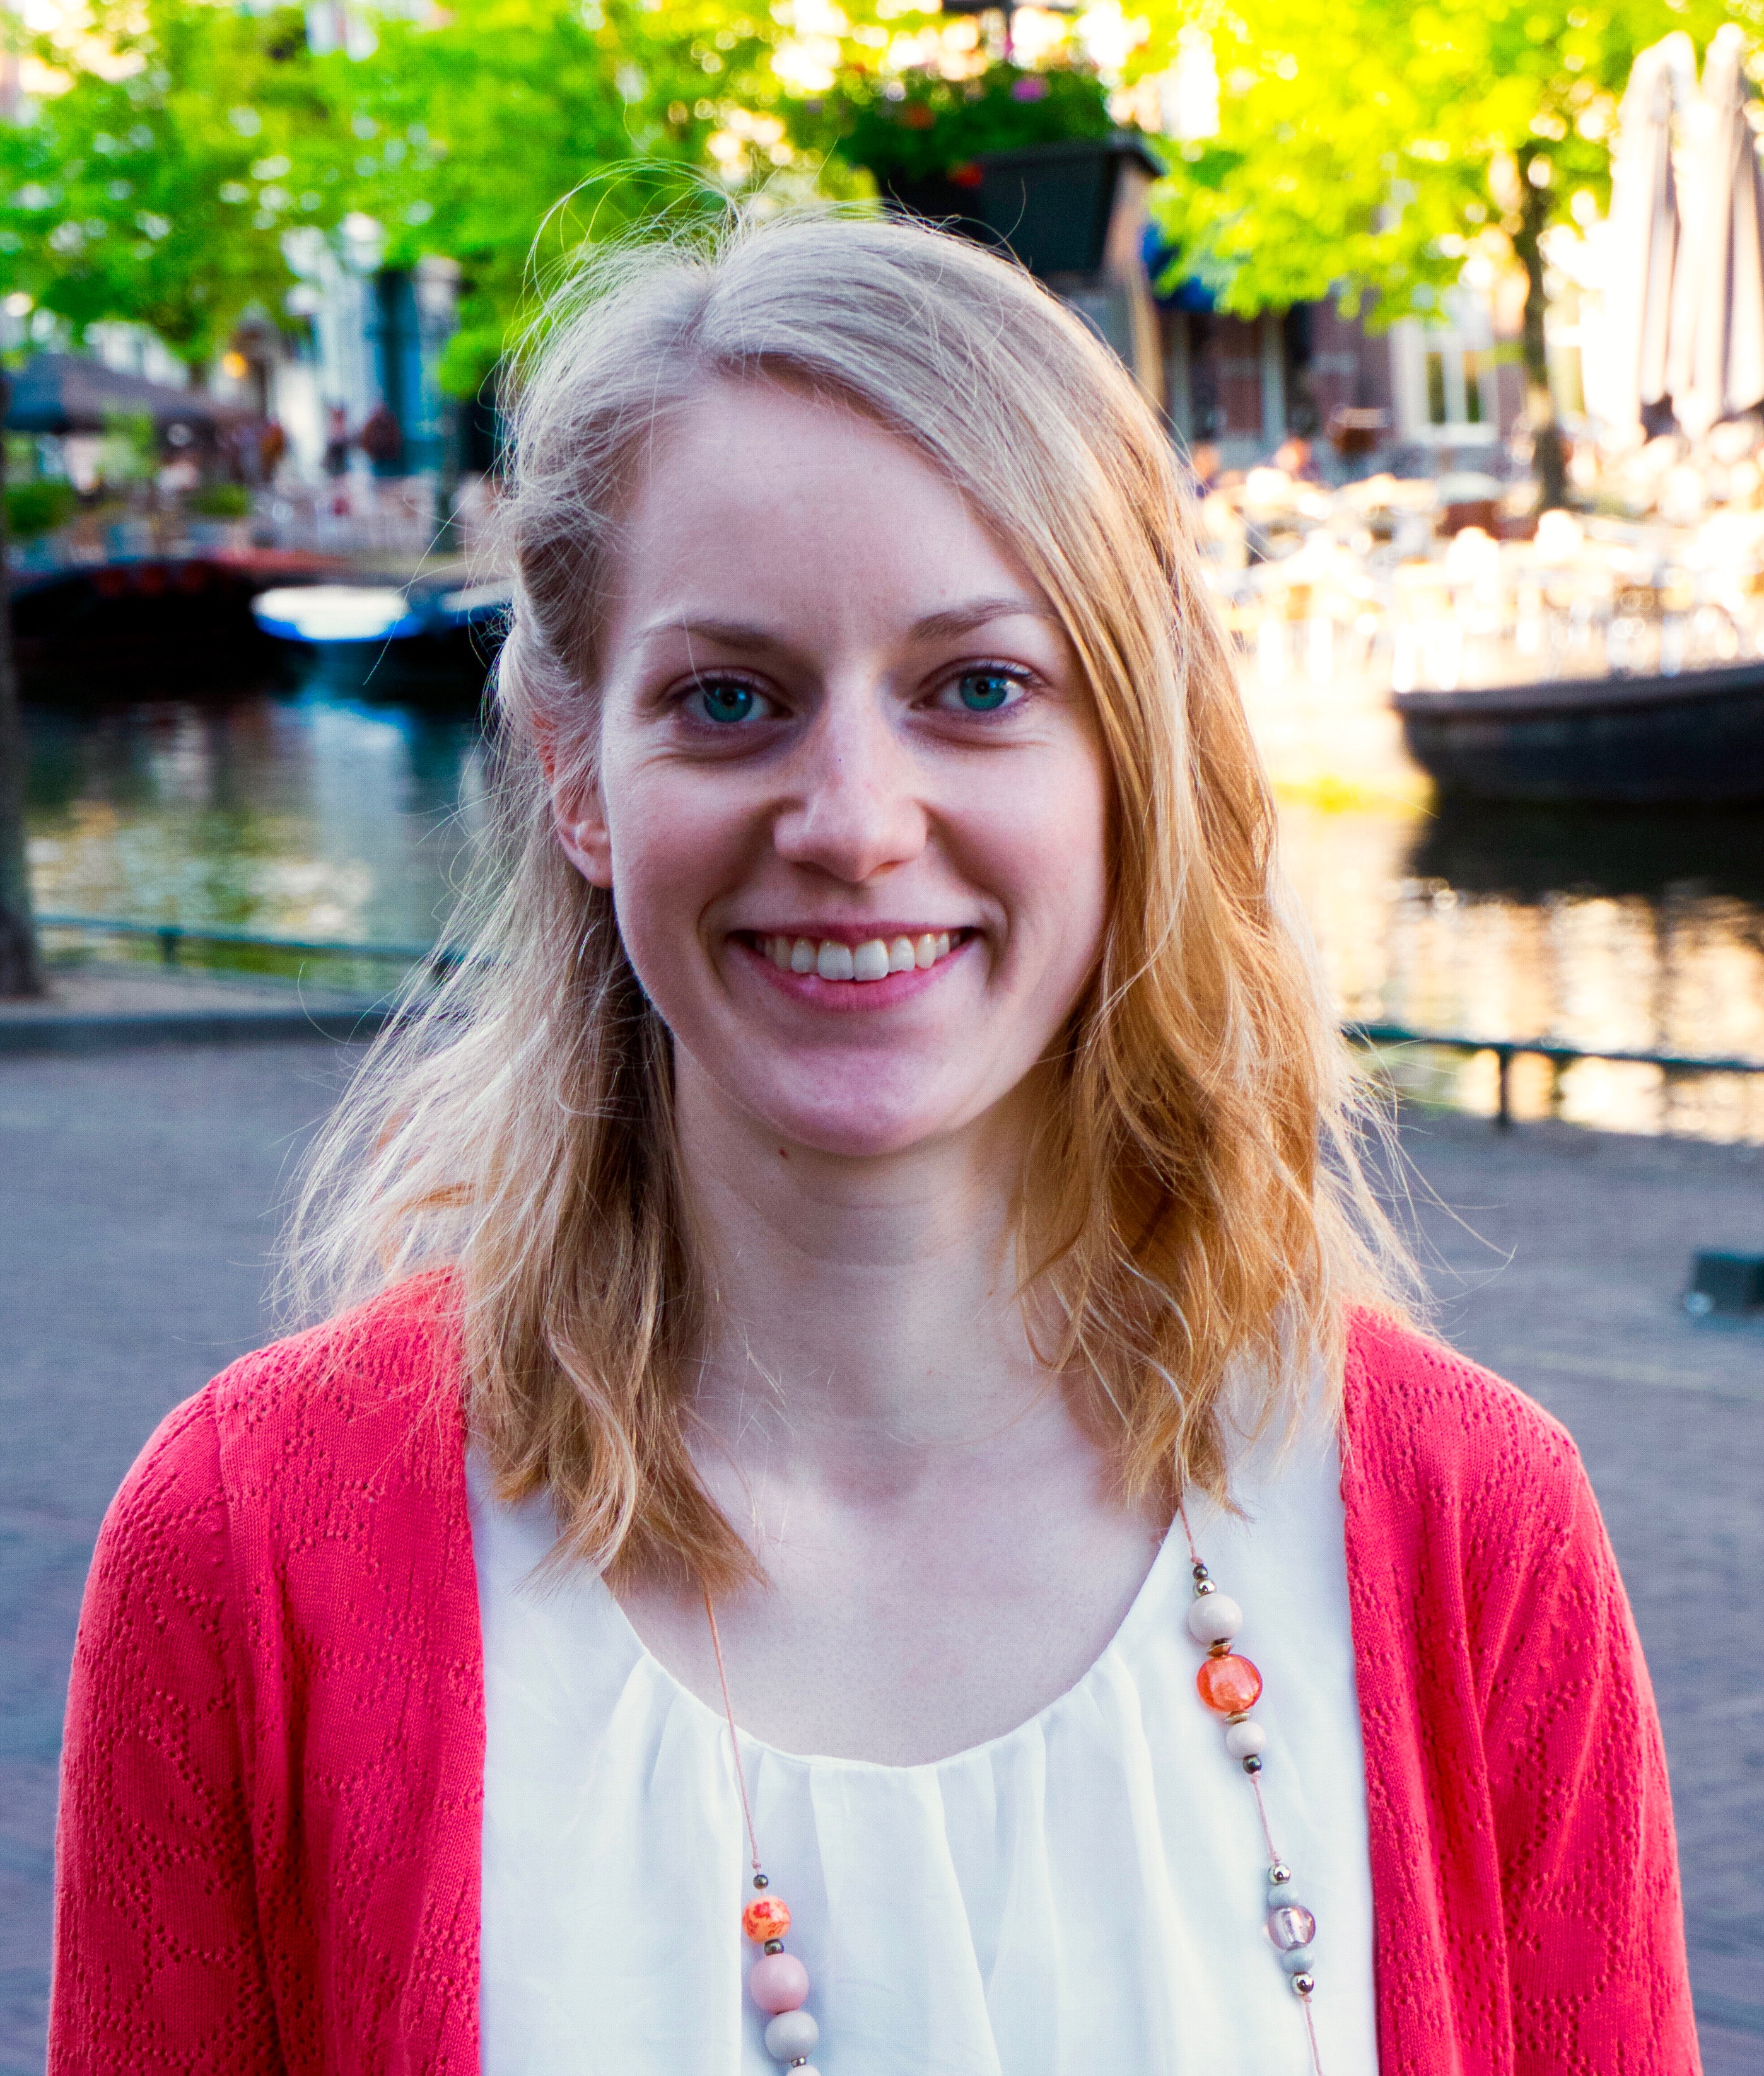
\includegraphics[width=\columnwidth,height=\paperheight,keepaspectratio]{../pictures/marthe.jpg}}
		\column{.7\textwidth}
		dr. A. Marthe Möller \\
		Assistant Professor Entertainment Communication
		\begin{itemize}
			\item Studying entertainment experiences in the digital space using:
			\begin{itemize}
				\item Computational methods (e.g., ACA of user comments)
				\item Experimental methods
			\end{itemize}
		\end{itemize}
		@marthemoller \textbar a.m.moller@uva.nl \textbar \url{https://www.uva.nl/profiel/m/o/a.m.moller/a.m.moller.html} 
	\end{columns}
\end{frame}

\begin{frame}{Introducing\ldots \huge{Anne}} 
	\begin{columns}[] \column{.3\textwidth} \makebox[\columnwidth]{ 
\includegraphics[width=\columnwidth,height=\paperheight,keepaspectratio]{../pictures/anne.jpg}} \column{.7\textwidth} dr. Anne Kroon \\ 
		Associate Professor Corporate Communication
		\begin{itemize} 
			\item Research focus on biased AI in recruitment, and media bias regarding minorities
			\item Text analysis using automated approaches, word embeddings
		\end{itemize} @annekroon \textbar a.c.kroon@uva.nl  \textbar \\ \url{http://www.uva.nl/profiel/k/r/a.c.kroon/a.c.kroon.html} 
	\end{columns} 
\end{frame}

\section[The course]{Introducing\ldots the course}

\begin{frame}{About CCS-2} 
What is CCS-2?
	\begin{itemize}
		\item Next step after CCS-1 
		\item Learn how to use what you learned in CCS-1 for research
		\item Expand on what you learned in CCS-1
		\begin{itemize}
			\item Learn computational techniques (e.g. data vectorization, machine learning)
			\item Learn how to use these techniques for research (e.g., automated content analysis)
		\end{itemize}
		\item By the end of the course, you'll be prepared for the \emph{Research Project}
	\end{itemize}
	
\end{frame}

\begin{frame}{About CCS-2}
	\begin{center}
		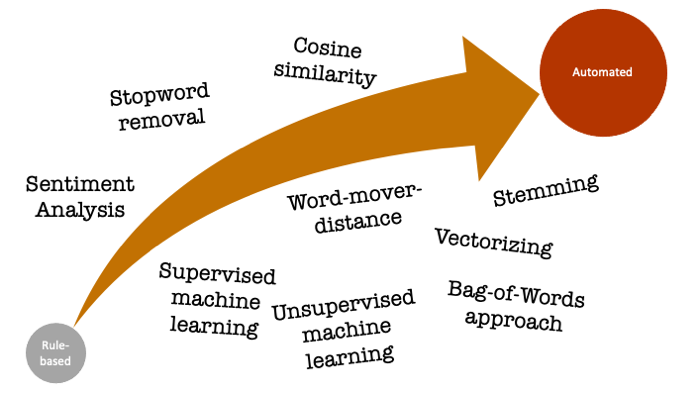
\includegraphics[width=\linewidth,height=\textheight,keepaspectratio]{../pictures/Roadmap_terms.png} 
	\end{center}
\end{frame}


\begin{frame}{About CCS-2} 

What will we do in this course?	
	\begin{itemize}[<+->]
		\item We discuss techniques in the lectures (Mondays)
		\item We practice with techniques in the tutorials (Tuesdays)
		\item Graded assignments to master the techniques:
		\begin{itemize}
			\item Regular multiple choice questions (\(20\%\)) about the readings and techniques that we discuss
			\begin{itemize}
				\item 4 questions, in week 2, 3, 4, 6, 7 
				\item \emph{total of 20 questions. 16 correct answers = full marks}
			\end{itemize}
			\item Group assignment: Get more experienced with the techniques and build a \emph{basic} recommender system
			\begin{itemize}
				\item Written report and code assignment (\(30\%\))
			\end{itemize}
			\item Final assignment (\(50\%\)): at the end of the course so you can show off what you learned
		\end{itemize}
		\item We provide structure through the meetings and assignments, you do the (home-)work
	\end{itemize}
	
\end{frame}

\begin{frame}{About CCS-2} 
	
Course set-up:
\begin{itemize}[<+->]
	\item \emph{Lectures}: Introduction to techniques used in computational communication science
	\item \emph{Tutorial meetings}: Lab sessions to learn how to work with these techniques
	\begin{itemize}
		\item Possibility to ask questions about your code
	\end{itemize}
\end{itemize}

\end{frame}

\begin{frame} 
	All course materials can be found at\ldots \\
	~~~~~~~~\url{https://github.com/uva-cw-ccs2/2324s2}
\end{frame}

\begin{frame}{About CCS-2} 
How to stay informed and where to find all the materials? Regularly check:	
	\begin{itemize}
		\item The course Canvas page
		\item Your email
		\item The course Github page
	\end{itemize}
In addition, make sure that you read the course manual so that you know all the ins and outs of this course!
\end{frame}


\begin{frame}{Ready? Set? Go!} 
	
	Without further ado\dots
	
	\dots let's get started!
	
\end{frame}

\section{Text as data}

\begin{frame}{Text as Data}
	CCS-1: You learned how to...
		\begin{itemize}
		\item Work with Python, for example, you:
		\begin{itemize}
			\item Store text in json-files, csv-files etc.
			\item Difference between a dict, a list, a string etc.
			\item Work with data (e.g., creating a loop)
		\end{itemize}
	\end{itemize}
	\end{frame}

\begin{frame}{Text as Data: Analyzing text as a goal}
	Studying text can teach us a lot about human behavior:
	\begin{itemize}[<+->]
	\item \dots to study the content cancer-related online platforms (e.g., \cite{sanders_different_2020})
	\begin{itemize}
	\item what \emph{topics} are being discussed on expert and peer-generated platforms?
	\end{itemize}
	\item \dots does content differ between online and print news? (e.g., \cite{burggraaff_through_2020})
	\begin{itemize}
	\item E.g., online, journalists are more likely to publish \emph{follow-up} articles.
	\end{itemize}
	\end{itemize}
\end{frame}
	
\begin{frame}{Text as Data: Analyzing text as a means}
Studying text can give us information we can use to answer broader questions: 
\begin{itemize}[<+->]
	\item \dots analyze textual information about movies from IMDB to learn about the representation of women in movies (e.g.,\cite{poma-murialdo_gender_2019} )
	\item \dots automatically distinguish between reliable and unreliable online information about vaccines 
	by investigating what characterizes reliable and unreliable texts (e.g.,\cite{meppelink_reliable_2021})
\end{itemize}
\end{frame}

\begin{frame}{Text as data: NLP}
\alert{Natural language processing (NLP)} refers to the branch of computer science — and more specifically, the branch of artificial intelligence or AI — concerned with giving computers the ability to understand text and spoken words in much the same way human beings can."  \\
\tiny{(IBM, 2020)}
\\ \\
Watch this Ted talk for some inspiration if you like: 
\url{https://www.ted.com/talks/jean_baptiste_michel_erez_lieberman_aiden_what_we_learned_from_5_million_books}
\end{frame}


\section{The toolkit}
\subsection{Bottom-up vs. top-down}

\begin{frame}[standout]
	Automated content analysis can be either \textcolor{red}{bottom-up} (inductive, explorative, pattern recognition, \ldots) or \textcolor{red}{top-down} (deductive, based on a-priori developed rules, \ldots). Or in between.
\end{frame}

\begin{frame}{The CCS toolbox}
	\makebox[\columnwidth]{
		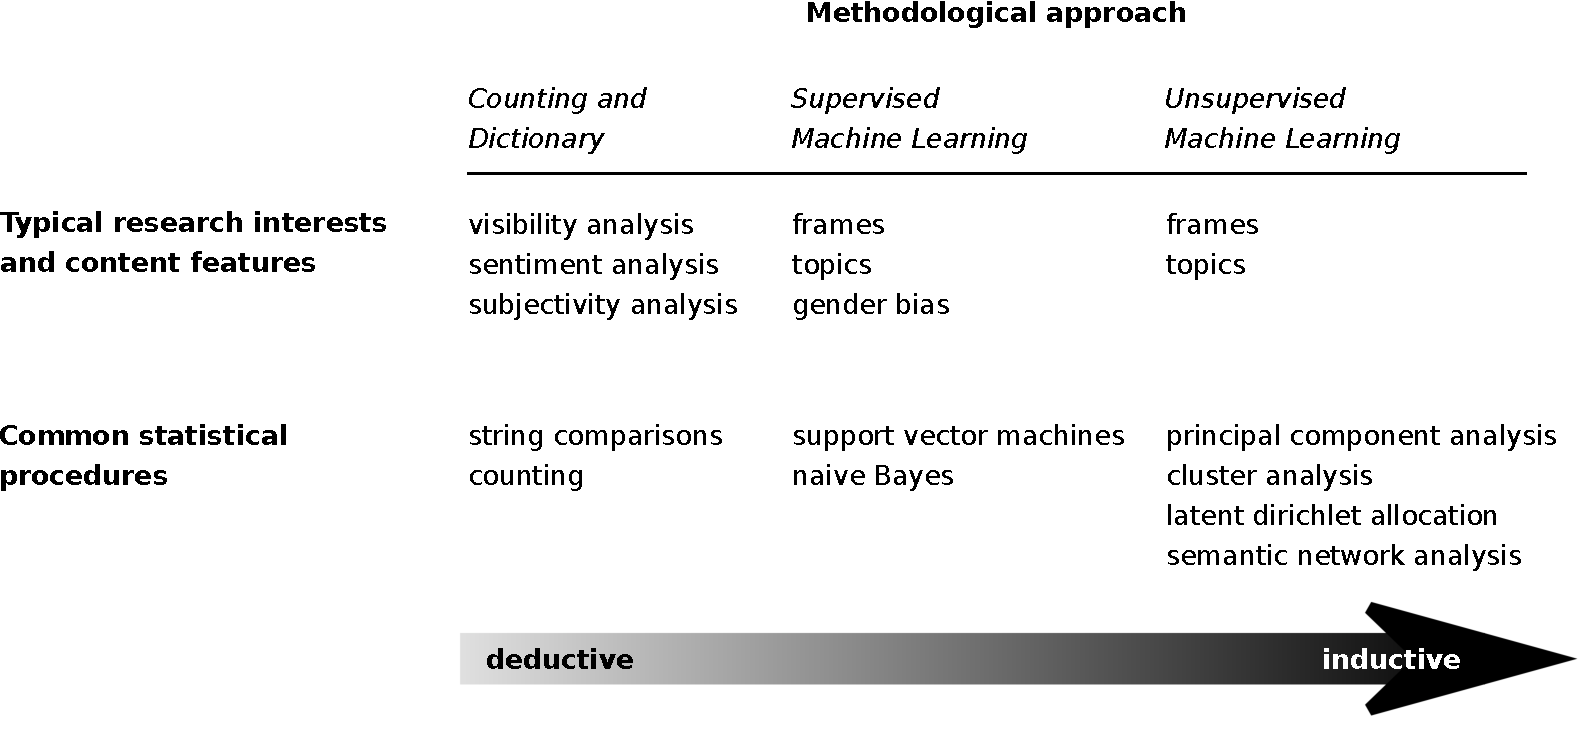
\includegraphics[width=\columnwidth,height=\paperheight,keepaspectratio]{../pictures/boumanstrilling2016}}
	\\
	\cite{Boumans2016}
\end{frame}

\begin{frame}{Bottom-up vs. top-down}
	\begin{block}{Bottom-up}
		\begin{itemize}
			\item Count most frequently occurring words 
			\item Maybe better: Count combinations of words $\Rightarrow$ Which words co-occur together?
		\end{itemize}
		We \emph{don't} specify what to look for in advance	
	\end{block}
	
	\onslide<2>{
		\begin{block}{Top-down}
			\begin{itemize}
				\item Count frequencies of pre-defined words
				\item Maybe better: patterns instead of words
			\end{itemize}
			We \emph{do} specify what to look for in advance	
		\end{block}
	}
\end{frame}

\begin{frame}[fragile]{A simple bottom-up approach}
\begin{minted}[%
	breaklines,
	linenos,
	fontsize=\scriptsize,
	frame=single,
	xleftmargin=0pt,]
	{python}
from collections import Counter
texts = ["Communication in the Digital Society is a very very complex phenomenon", "I like to study it"]
bottom_up = []
for t in texts:
    bottom_up.append(Counter(t.lower().split()).most_common(3))
print(bottom_up)
\end{minted}
\pause
This results in:
\begin{minted}[fontsize=\scriptsize]{python}
[('very', 2), ('Communication', 1), ('in', 1)]
[('I', 1), ('like', 1), ('to', 1)]
\end{minted}
\textcolor{red}{\footnotesize{\emph{Please note that you can also write this like:}}}
\pause
\begin{minted}[%
	breaklines,
	linenos,
	fontsize=\scriptsize,
	frame=single,
	xleftmargin=0pt,]
	{python}
bottom_up = [Counter(t.split()).most_common(3) for t  in texts]
\end{minted}
\begin{itemize}
\tiny{
	\item This is \emph{exactly} the same, just shorter (and faster). 
	\item You do \emph{not} have to use list comprehensions, but it helps if you can read them. }
\end{itemize}
\end{frame}

\begin{frame}[fragile]{A simple top-down approach}
\begin{minted}[%
	breaklines,
	linenos,
	fontsize=\scriptsize,
	frame=single,
	xleftmargin=0pt,]
	{python}
texts = ["Communication in the Digital Society is a very very complex phenomenon", "I like to study it"]
features = ["communication", "digital", "study"]
for t in texts:
    print(f"\nAnalyzing '{t}':")
       for f in features:
          print(f"{f} occurs {t.lower().count(f)} times")
\end{minted}
\pause
\begin{minted}[%
	frame=none,
	framesep=1mm,
	baselinestretch=1,
	bgcolor=listingbg,
	linenos,
	breaklines,
	fontsize=\tiny]{python}
Analyzing 'Communication in the Digital Society is a very very complex phenomenon':
communication occurs 1 times
digital occurs 1 times
study occurs 0 times

Analyzing 'I like to study it':
communication occurs 0 times
digital occurs 0 times
study occurs 1 times	
\end{minted}
\pause
\textcolor{red}{\footnotesize{\emph{\dots save the results as a \texttt{list} as follows \dots}}}
\pause
\begin{minted}[%
	breaklines,
	linenos,
	fontsize=\tiny,
	frame=single,
	xleftmargin=0pt,]
	{python}
top_down = [[t.lower().count(f) for f in features] for t in texts]
\end{minted}
\end{frame}

\question{When would you use which approach?}

\begin{frame}{Some considerations}
	\begin{itemize}[<+->]
		\item Both can have a place in your workflow (e.g., bottom-up as first exploratory step)
		\item You have a clear theoretical expectation? Bottom-up makes little sense.
		\item But in any case: you need to transform your text into something ``countable''.
	\end{itemize}
\end{frame}

\section{Preprocessing}

\begin{frame}
	\begin{block}{Preprocessing in NLP}
		\begin{itemize}	
	\item Text preprocessing in \emph{Natural Language Processing}. 
	\item Typical step to get textual data into a more structured format for subsequent analyses
	\item These steps will come back in the upcoming weeks when we discuss bottom-up and top-down techniques
		\end{itemize}
\end{block}
\end{frame}

\begin{frame}{Typical preprocessing steps}
	\begin{block}{Preprocessing steps}
		\begin{description}
			\item [\emph{tokenization}] How do we (best) split a sentence into tokens (terms, words)?
			\item [\emph{pruning}] How can we remove unneccessary words/ punctuation?
			\item [\emph{lemmatization and stemming}] How can we make sure that slight variations of the same word are not counted differently?
			\item [\emph{ngrams}] Neighbouring terms
		\end{description}
	\end{block}
\end{frame}

\begin{frame}[fragile]{Simple string methods}
	\begin{block}{Slicing}
		\texttt{mystring[2:5]} to get the characters with indices 2,3,4
	\end{block}
	\begin{block}{String methods}
		\begin{itemize}
			\item \texttt{.lower()} returns lowercased string
			\item \texttt{.strip()} returns string without whitespace at beginning and end
			\item \texttt{.find("bla")} returns index of position of substring ``bla'' or -1 if not found
			\item \texttt{.replace("a","b")} returns string where "a" is replaced by "b"
			\item \texttt{.count("bla")} counts how often substring ``bla'' occurs
		\end{itemize}
		Use tab completion for more!
	\end{block}
\end{frame}

%\subsection*{Tokenization}

\begin{frame}[fragile]{OK, good enough, perfect?}
	\begin{block}{.split()}
		\begin{itemize}
			\item space $\rightarrow$ new word
			\item no further processing whatsoever
			\item thus, only works well if we do a preprocessing outselves (e.g., remove punctuation)
		\end{itemize}
	\end{block}
\pause
\begin{minted}[%
	breaklines,
	linenos,
	fontsize=\scriptsize,
	frame=single,
	xleftmargin=0pt,]
	{python}
docs = ["This is a text",  "I haven't seen John's derring-do. Second sentence!"]
tokens = [d.split() for d in docs]
\end{minted}
	
\begin{minted}[%
	fontsize=\scriptsize,]
	{python}
[['This', 'is', 'a', 'text'], ['I', "haven't", 'seen', "John's", 
'derring-do.', 'Second', 'sentence!']]
\end{minted}
\end{frame}

\begin{frame}[fragile]{OK, good enough, perfect?}
	\begin{block}{Tokenizers from the NLTK package}
		\begin{itemize}
			\item multiple improved tokenizers that can be used instead of .split()
			\item e.g., Treebank tokenizer:
			\begin{itemize}
				\item split standard contractions ("don't")
				\item deals with punctuation
			\end{itemize}			
		\end{itemize}
	\end{block}
\pause
\begin{minted}[%
	breaklines,
	linenos,
	fontsize=\scriptsize,
	frame=single,
	xleftmargin=0pt,]
	{python}
from nltk.tokenize import TreebankWordTokenizer
tokens = [TreebankWordTokenizer().tokenize(d) for d in docs]
\end{minted}
\pause
\begin{minted}[%
breaklines,
fontsize=\scriptsize]
{python}
[['This', 'is', 'a', 'text'],  ['I', 'have', "n't", 'seen', 'John', "'s", 'derring-do.', 'Second', 'sentence', '!']]
\end{minted}
\tiny{Notice the failure to split the \texttt{.} at the end of the first sentence in the second doc. That's because \texttt{TreebankWordTokenizer} expects \emph{sentences} as input. See book for a solution.\\}
\end{frame}

%\subsection*{Stopword and punctuation removal}

\begin{frame}
	\textbf{Stopword removal} \\
	\vspace{1cm}
	\begin{itemize}
		\item <2->{\emph{The logic of the algorithm is very much related to the one of a simple sentiment analysis!}}
	\end{itemize}
\end{frame}

\begin{frame}{Stopword removal}
	\begin{block}{What are stopwords?}
		\begin{itemize}
			\item Very frequent words with little inherent meaning
			\item \texttt{the, a, he, she, \ldots}
			\item context-dependent: if you are interested in gender, \texttt{he} and \texttt{she} are no stopwords. 
			\item Many existing lists as basis
		\end{itemize}
	\end{block}
	
\end{frame}

\begin{frame}{Stopword removal: What and why?}
	\begin{block}{Why remove stopwords?}
		\begin{itemize}
			\item If we want to identify key terms (e.g., by means of a word count), we are not interested in them
			\item If we want to calculate document similarity, it might be inflated
			\item If we want to make a word co-occurance graph, irrelevant information will dominate the picture
		\end{itemize}
	\end{block}
\end{frame}

\begin{frame}[fragile]{Stopword removal}
\begin{minted}[%
	breaklines,
	linenos,
	fontsize=\scriptsize,
	frame=single,
	xleftmargin=0pt,]
	{python}
from nltk.corpus import stopwords
mystopwords = stopwords.words("english")
mystopwords.extend(["test", "this"])

tokens_without_stopwords = [[word for word in doc if word.lower() not in mystopwords] for doc in tokens]
\end{minted}
\begin{minted}[%
fontsize=\scriptsize,]
{python}
[['text'], ["n't", 'seen', 'John', 'derring-do.', 'Second', 'sentence', '!']]
\end{minted}
	
\begin{alertblock}{You can do more!}
		\tiny{For instance, you could add an \texttt{or} statement to also exclude punctuation.}
\end{alertblock}
	
\end{frame}

\begin{frame}[fragile]{Removing punctuation}
\begin{minted}[%
	breaklines,
	linenos,
	fontsize=\scriptsize,
	frame=single,
	xleftmargin=0pt,]
	{python}
from nltk.tokenize import RegexpTokenizer
tokenizer = RegexpTokenizer(r'\w+')
tokenizer.tokenize("Hi students, what's up!")
\end{minted}
\pause
\begin{minted}[%
	fontsize=\scriptsize,]
	{python}
['Hi', 'students', 'what', 's', 'up']
\end{minted}	
\end{frame}

%\subsection*{Stemming and lemmatization}

\begin{frame}{Stemming and lemmatization}
\begin{block}{Why do we need this?}
	\begin{itemize}
		\item Because we do not want to distinguish between smoke, smoked, smoking, \ldots
		\item Typical preprocessing step (like stopword removal)
		\item Ultimate aim: normalize text
	\end{itemize}
\end{block}
\end{frame}

\begin{frame}[fragile]{Stemming}
\begin{itemize}
\item Stemming: reduce words to its stem by removing last part (drinking $\rightarrow$ drink)
\end{itemize}
\pause
\begin{itemize}
\item Lemmatization: find word that you would need to look up in a dictionary (drinking $\rightarrow$ drink, but also went $\rightarrow$ go)
\item stemming is simpler than lemmatization
\item lemmatization often better
\end{itemize}
\end{frame}

%\begin{frame}[fragile]{Stemming and Lemmatizing}
\begin{minted}[%
	breaklines,
	linenos,
	fontsize=\tiny,
	frame=single,
	xleftmargin=0pt,]
	{python}
import nltk
import spacy
porter_stemmer = nltk.stem.PorterStemmer() # NLTK's Porter Stemmer
nlp = spacy.load("en_core_web_sm")# Load spaCy's English language model
sentence = "The dogs are barking, the cats are playing, the girl sang a song"
# Use NLTK's Porter Stemmer to stem the sentence
stemmed_sentence = " ".join([porter_stemmer.stem(word) for word in sentence.split()])
# Use spaCy's English language model to lemmatize the sentence
lemmatized_sentence = " ".join([token.lemma_ for token in nlp(sentence)])
# Print the original sentence, stemmed sentence, and lemmatized sentence
print(sentence)
print(stemmed_sentence)
print(lemmatized_sentence)
\end{minted}

\begin{minted}[%
	breaklines,
	linenos,
	fontsize=\tiny,
	frame=single,
	xleftmargin=0pt,]
	{python}
The dogs are barking, the cats are playing, the girl sang a song
the dog are barking, the cat are playing, the girl sang a song
the dog be bark , the cat be play , the girl sing a song
\end{minted}
\end{frame}

%\subsection*{Ngrams}

\begin{frame}{ngrams}
	Instead of just looking at single words (unigrams), we can also use adjacent words (bigrams).
\end{frame}

\begin{frame}[fragile]{ngrams}
\begin{minted}[%
	breaklines,
	linenos,
	fontsize=\scriptsize,
	frame=single,
	xleftmargin=0pt,]
	{python}
import nltk
texts = ['This is the first text text text first', 'And another text yeah yeah']
texts_bigrams = [["_".join(tup) for tup in nltk.ngrams(t.split(),2)] for t in texts]
print(texts_bigrams)
\end{minted}

\texttt{[['This\_is',
	'is\_the',
	'the\_first',
	'first\_text',
	'text\_text',
	'text\_text',
	'text\_first'],
	['And\_another', 'another\_text', 'text\_yeah', 'yeah\_yeah']] }

Typically, we would combine both uni and bigrams. 

	\pause
	\textbf{\textcolor{red}{What do you think? Why is this useful? (and what may be drawbacks?)}}
\end{frame}

\begin{frame}{Main takeaway}
	\begin{itemize}
		%	\item It matters how you transform your text into numbers (``vectorization'').
		\item Preprocessing matters, be able to make informed choices.
		\item Keep this in mind when moving to Machine Learning. 
	\end{itemize}
\end{frame}

\section{From test to large-scale}

\begin{frame}[fragile]{General approach}
1. Take a single string and test your idea
\begin{minted}[%
	breaklines,
	linenos,
	fontsize=\scriptsize,
	frame=single,
	xleftmargin=0pt,]
	{python}
t = "This is a test test test."
print(t.count("test"))
\end{minted}
2a. You'd assume it to return 3. If so, scale it up:
\pause
\begin{minted}[%
	breaklines,
	linenos,
	fontsize=\scriptsize,
	frame=single,
	xleftmargin=0pt,]
	{python}
results = []
for t in listwithallmytexts:
    r = t.count("test")
    print(f"{t} contains the substring {r} times")
	results.append(r)
\end{minted}

2b. If you \emph{only} need to get the list of results, a list comprehension is more elegant:
\begin{minted}[%
	breaklines,
	linenos,
	fontsize=\scriptsize,
	frame=single,
	xleftmargin=0pt,]
	{python}
results = [t.count("test") for t in listwithallmytexts]
\end{minted}


\end{frame}

\begin{frame}[fragile]{General approach}
\Large

\textcolor{red}{Test on a single string, then make a for loop or list comprehension!}

\pause

\normalsize

\begin{alertblock}{Own functions}
	If it gets more complex, you can write your ow= function and then use it in the list comprehension:
\begin{minted}[%
	breaklines,
	linenos,
	fontsize=\scriptsize,
	frame=single,
	xleftmargin=0pt,]
	{python}
def mycleanup(t):
     # do sth with string t here, create new string t2
     return t2
		
results = [mycleanup(t) for t in allmytexts]
\end{minted}
\end{alertblock}
\end{frame}


\begin{frame}[fragile]{Pandas string methods as alternative}
If you select column with strings from a pandas dataframe, pandas offers a collection of string methods (via \texttt{.str.}) that largely mirror standard Python string methods:

\begin{minted}[%
	breaklines,
	linenos,
	fontsize=\scriptsize,
	frame=single,
	xleftmargin=0pt,]
	{python}
df['newcoloumnwithresults'] = df['columnwithtext'].str.count("bla")
\end{minted}


\pause

\begin{alertblock}{To pandas or not to pandas for text?}
	Partly a matter of taste. 
	
	Not-too-large dataset with a lot of extra columns? Advanced statistical analysis planned? Sounds like pandas.
	
	It's mainly a lot of text? Wanna do some machine learning later on anyway? It's large and (potentially) messy? Doesn't sound like pandas is a good idea.
\end{alertblock}

\end{frame}

\begin{frame}{Tuesday April 2}
	\begin{block}{Tutorial meeting tomorrow}
		\begin{itemize}
			\item Start to practice with preprocessing techniques yourself
			\item Try the code in these slides at home. Make sure you can follow along.
			\item Use the tutorial meetings to discuss your questions.
		\end{itemize}
	\end{block}
\end{frame}

\begin{frame}{Practice is key!}
    \centering
    
\includegraphics[width=0.8\textwidth,height=0.8\textheight,keepaspectratio]{python_running.jpeg}
    %\footnote{https://towardsdatascience.com/what-is-cosine-similarity-how-to-compare-text-and-images-in-python-d2bb6e411ef0}
\end{frame}


\begin{frame}{Thank you!!}
	\begin{block}{Thank you for your attention!}
		\begin{itemize}
			\item Questions? Comments?
		\end{itemize}
	\end{block}
\end{frame}

\begin{frame}[t,allowframebreaks]
	\frametitle{References}
	\printbibliography
\end{frame}

\end{document}